\documentclass[12pt,a4paper]{article}

\usepackage[utf8]{inputenc}
\usepackage[T1]{fontenc}
\usepackage[provide=*,brazilian]{babel}
\usepackage{lmodern}
\usepackage{geometry}
\usepackage{setspace}
\usepackage{indentfirst}
\usepackage{graphicx}
\usepackage{amsmath}
\usepackage{booktabs}
\usepackage{longtable}
\usepackage{tabularx}
\usepackage{array}
\usepackage{float}
\usepackage{caption}
\usepackage{enumitem}
\usepackage{xcolor}
\usepackage{microtype}
\usepackage{csquotes}
\usepackage{fancyhdr}
\usepackage{hyperref}
\usepackage{tikz}

\usetikzlibrary{arrows.meta,positioning,shapes.geometric}

\geometry{top=3cm,left=3cm,right=2cm,bottom=2cm}
\onehalfspacing
\setlength{\parindent}{1.25cm}
\setlength{\parskip}{0pt}
\setlist{nosep,leftmargin=1.25cm}
\setlength{\emergencystretch}{2em}

\definecolor{melodyblue}{HTML}{174A7E}
\definecolor{melodygreen}{HTML}{207A5B}
\definecolor{melodyred}{HTML}{A73939}

\hypersetup{
    colorlinks=true,
    linkcolor=melodyblue,
    citecolor=melodygreen,
    urlcolor=melodyblue,
    pdftitle={Melody: reconhecimento de músicas utilizando Raspberry Pi 3},
    pdfauthor={Ana Vitória Abreu Murad, Andrey Rocha Reboredo e Yasmin Francisquetti Barnes}
}
\urlstyle{same}

\newcolumntype{Y}{>{\raggedright\arraybackslash}X}
\newcolumntype{C}[1]{>{\centering\arraybackslash}p{#1}}
\newcommand{\codigo}[1]{\texttt{#1}}
\newcommand{\caminho}[1]{\nolinkurl{#1}}
\newcommand{\VideoFinalURL}{\href{https://drive.google.com/drive/folders/1zcMDBFCq20FDo9gOkV1ytAR7sOgkPn05?usp=sharing}{pasta da demonstração final no Google Drive}}

\pagestyle{fancy}
\fancyhf{}
\fancyhead[L]{PCS3732 --- Laboratório de Processadores}
\fancyhead[R]{Melody}
\fancyfoot[C]{\thepage}
\setlength{\headheight}{15pt}

\begin{document}

\hypersetup{pageanchor=false}
\begin{titlepage}
    \centering
    \textbf{UNIVERSIDADE DE SÃO PAULO}\\
    \textbf{ESCOLA POLITÉCNICA}\\
    Departamento de Engenharia de Computação e Sistemas Digitais\\[1.2cm]

    
\includegraphics[width=3.1cm]{song-recognizer/src/interface/static/images/melody_logo.png}\\[0.8cm]

    {\Large\textbf{MELODY: RECONHECIMENTO DE MÚSICAS\\
    UTILIZANDO RASPBERRY PI 3}}\\[1.2cm]

    {\large Relatório final do projeto}\\[1.2cm]

    \begin{tabular}{c}
        Ana Vitória Abreu Murad\\
        Andrey Rocha Reboredo\\
        Yasmin Francisquetti Barnes
    \end{tabular}

    \vfill
    Relatório apresentado à disciplina PCS3732 --- Laboratório de Processadores.\\[1.2cm]

    São Paulo\\
    2026
\end{titlepage}
\hypersetup{pageanchor=true}

\pagenumbering{roman}

\section*{Resumo}
\addcontentsline{toc}{section}{Resumo}

Este trabalho apresenta o desenvolvimento do Melody, um reconhecedor de músicas
executado localmente em uma Raspberry Pi 3 B+. O sistema grava oito segundos de
áudio por um microfone USB, normaliza o sinal, calcula uma Transformada de Fourier
de Curto Termo, seleciona máximos locais do espectrograma e produz impressões
digitais acústicas a partir de pares de picos. Os hashes são comparados com um
banco SQLite por votação de deslocamentos temporais. A solução inclui interface
web local, controles físicos conectados aos pinos GPIO, cadastro automatizado de
músicas e cancelamento imediato da execução. Ao final do projeto, o banco continha
11 músicas e 300.057 fingerprints. Um benchmark determinístico avaliou 99 trechos
de músicas cadastradas, incluindo áudio limpo, ruído e eco, e obteve 99 acertos.
Em contraste, três sinais sintéticos desconhecidos não foram rejeitados, o que
evidencia a necessidade de calibrar um limiar mínimo de aceitação. Na demonstração
final, a gravação cadastrada de “I'm a Believer” foi reconhecida, enquanto uma
versão cover e uma interpretação de outro artista não foram identificadas. Os
resultados confirmam a viabilidade do processamento offline no hardware adotado,
mas também delimitam o protótipo ao reconhecimento de gravações específicas.

\noindent\textbf{Palavras-chave:} reconhecimento de músicas; impressão digital
acústica; STFT; Raspberry Pi; sistemas embarcados.

\section*{Abstract}
\addcontentsline{toc}{section}{Abstract}

This report presents Melody, an offline song-recognition system running on a
Raspberry Pi 3 B+. The system records an eight-second audio excerpt through a USB
microphone, preprocesses the signal, computes a Short-Time Fourier Transform,
selects local spectrogram peaks, and creates acoustic fingerprints from peak
pairs. The hashes are matched against a local SQLite database through temporal
offset voting. The final prototype includes a local web interface, GPIO controls,
automated song registration, and immediate execution cancellation. Its database
contains 11 songs and 300,057 fingerprints. A deterministic benchmark evaluated
99 registered-song excerpts under clean, noisy, and echo conditions and correctly
identified all of them. However, none of three synthetic unknown signals was
rejected, showing that a calibrated acceptance threshold is still required. In
the final demonstration, the registered recording of “I'm a Believer” was
recognized, whereas a cover and a version by another artist were not. The results
support the feasibility of offline embedded recognition while confirming that the
prototype identifies specific recordings rather than compositions in general.

\noindent\textbf{Keywords:} song recognition; acoustic fingerprinting; STFT;
Raspberry Pi; embedded systems.

\tableofcontents
\clearpage
\pagenumbering{arabic}

\section{Introdução}

O reconhecimento automático de músicas é uma aplicação de recuperação de
informação capaz de associar um pequeno trecho de áudio a uma gravação previamente
conhecida. A tarefa combina aquisição de sinais, processamento digital, extração
de características, indexação e busca. Serviços comerciais demonstram que a
identificação pode permanecer funcional mesmo quando o trecho é capturado por um
microfone e contém ruído ou não começa no mesmo instante da referência
\cite{wang2003}.

O projeto Melody transpõe esse problema para uma plataforma embarcada de recursos
limitados. Em vez de enviar áudio a um serviço externo, toda a cadeia --- gravação,
processamento e consulta --- ocorre na Raspberry Pi e em um banco local. Essa
decisão permite estudar interfaces de hardware e software, mantém o funcionamento
sem Internet e torna cada etapa do algoritmo observável. A Raspberry Pi 3 B+
possui processador ARM Cortex-A53 de quatro núcleos a 1,4 GHz, 1 GB de memória e
cabeçalho GPIO de 40 pinos, características suficientes para o protótipo
\cite{raspberry2026}.

O trabalho foi desenvolvido na disciplina PCS3732 --- Laboratório de
Processadores, da Escola Politécnica da Universidade de São Paulo
\cite{usp2026}.

\subsection{Motivação e justificativa}

Além de sua utilidade cotidiana, o reconhecimento musical é um estudo de caso
adequado para a disciplina por integrar conceitos de sistemas microprocessados e
processamento de sinais. O projeto exercita captura por periférico USB, acesso a
GPIO, execução concorrente, persistência local e uma interface acessível por
navegador. A abordagem de impressões digitais acústicas também é mais compatível
com a Raspberry Pi 3 do que modelos extensos de aprendizado profundo: o banco é
precalculado e a consulta utiliza operações numéricas e buscas indexadas.

O sistema foi inspirado conceitualmente na estratégia de mapa de constelação e
alinhamento temporal descrita por Wang \cite{wang2003}. O objetivo, entretanto,
não é reproduzir a escala ou a robustez de um produto comercial, mas construir
uma implementação didática, verificável e extensível para um catálogo pequeno.

\subsection{Objetivos}

O objetivo geral é desenvolver um sistema embarcado capaz de identificar músicas
previamente cadastradas a partir de trechos capturados por microfone em uma
Raspberry Pi 3.

Os objetivos específicos são:

\begin{itemize}
    \item capturar e padronizar áudio em formato mono a 16 kHz;
    \item obter uma representação tempo--frequência por STFT;
    \item extrair picos espectrais e gerar fingerprints acústicos;
    \item armazenar metadados e fingerprints em banco local indexado;
    \item reconhecer trechos por colisão de hashes e alinhamento temporal;
    \item permitir o controle por interface web e botões GPIO;
    \item automatizar o cadastro de novas músicas e a execução de testes; e
    \item avaliar acertos, condições adversas, rejeição e cancelamento.
\end{itemize}

\subsection{Escopo}

O protótipo identifica a mesma gravação que foi cadastrada, mesmo quando a
consulta corresponde a outro ponto temporal ou contém perturbações moderadas. Ele
não foi projetado para reconhecer apenas a melodia, letra, canto, assobio ou
arranjos diferentes. Assim, a palavra “original” usada nos testes significa a
versão de referência presente no banco, e não necessariamente a primeira gravação
histórica da composição. Serviços em nuvem e catálogos externos também estão fora
do escopo.

\section{Fundamentação teórica}

\subsection{Amostragem e pré-processamento}

Um sinal de áudio digital pode ser representado pela sequência $x[n]$, obtida em
instantes igualmente espaçados. O Melody converte entradas para ponto flutuante,
combina canais em mono, remove amostras inválidas e componente contínua, reamostra
para 16 kHz e normaliza o pico. De acordo com o critério de Nyquist, essa taxa
representa frequências de até 8 kHz, intervalo suficiente para os picos utilizados
pelo sistema.

\subsection{DFT, FFT e STFT}

A Transformada Discreta de Fourier (DFT) de uma janela com $N$ amostras é

\begin{equation}
    X[k] = \sum_{n=0}^{N-1} x[n]e^{-j2\pi kn/N}, \qquad 0 \leq k < N.
    \label{eq:dft}
\end{equation}

A Transformada Rápida de Fourier (FFT) calcula a mesma DFT com decomposições que
reduzem a ordem de custo de $O(N^2)$ para $O(N\log N)$; a formulação de Cooley e
Tukey é uma referência clássica desse método \cite{cooley1965}. Como uma única
DFT perde a localização temporal das frequências, aplica-se uma janela móvel
$w[n]$, produzindo a Transformada de Fourier de Curto Termo:

\begin{equation}
    X(m,k) = \sum_{n=0}^{N-1} x[n+mH]w[n]e^{-j2\pi kn/N},
    \label{eq:stft}
\end{equation}

em que $m$ é o índice do quadro e $H$ é o avanço entre quadros. Na implementação,
$N=1024$, $H=256$, a janela é Hann e a FFT usa 2048 pontos. Em 16 kHz, isso
corresponde a janelas de 64 ms, avanço de 16 ms e espaçamento espectral de
aproximadamente 7,81 Hz. A magnitude é convertida para decibéis e normalizada em
relação ao maior bin:

\begin{equation}
    S_{\mathrm{dB}}(m,k)=20\log_{10}\!\left(
    \max(|X(m,k)|,\varepsilon)\right)-S_{\max}.
\end{equation}

\subsection{Mapa de constelação e fingerprints}

Armazenar todos os bins do espectrograma seria custoso e sensível a pequenas
variações. Em seu lugar, o algoritmo seleciona máximos locais entre 80 Hz e
7 kHz, acima de $-35$ dB. A vizinhança possui raio de 15 bins de frequência e
9 quadros no tempo, com limite de 30 picos por segundo. O resultado é um mapa de
constelação esparso, ilustrado na Figura~\ref{fig:espectrograma-landmarks}.

\begin{figure}[H]
    \centering
    \begin{minipage}[t]{0.49\textwidth}
        \centering
        
\includegraphics[width=\linewidth]{song-recognizer/plots/smash_mouth_i_m_believer_spectrogram.png}
        \small (a) Espectrograma logarítmico.
    \end{minipage}
    \hfill
    \begin{minipage}[t]{0.49\textwidth}
        \centering
        
\includegraphics[width=\linewidth]{song-recognizer/plots/smash_mouth_i_m_believer_landmarks.png}
        \small (b) Picos espectrais selecionados.
    \end{minipage}
    \caption{Representações intermediárias da gravação cadastrada de
    \emph{I'm a Believer}. Fonte: elaboração própria.}
    \label{fig:espectrograma-landmarks}
\end{figure}

Cada pico âncora de frequência $f_a$ é combinado com até cinco picos-alvo
$f_b$ localizados entre 0,1 s e 2,0 s depois dele. A chave antes do hash é

\begin{equation}
    K=(\lfloor f_a\rfloor,\lfloor f_b\rfloor,
    \operatorname{round}(1000\Delta t)).
\end{equation}

O SHA-1 de $K$ é calculado e truncado para 20 caracteres hexadecimais. O SHA-1 é
usado aqui apenas como função determinística e compacta de indexação, não como
mecanismo de segurança. Junto a cada hash é armazenado o instante da âncora.

\subsection{Correspondência por alinhamento temporal}

Para cada hash da consulta, o banco retorna ocorrências $(s,t_b)$, onde $s$ é a
música e $t_b$ é o instante na referência. Calcula-se

\begin{equation}
    \Delta=t_b-t_q,
\end{equation}

com arredondamento de 0,1 s. Hashes provenientes do mesmo trecho tendem a votar
no mesmo par $(s,\Delta)$, mesmo quando a consulta começa em outro ponto da
música. O par mais votado fornece a identificação e o deslocamento estimado.
Essa coerência temporal é mais discriminante do que a simples contagem de hashes
iguais \cite{wang2003}.

\section{Requisitos}

A Tabela~\ref{tab:requisitos} consolida os requisitos finais. Os testes associados
são detalhados na Seção~\ref{sec:testes}.

\begin{longtable}{C{1.25cm} p{6.1cm} p{6.1cm}}
    \caption{Requisitos funcionais e não funcionais.}\label{tab:requisitos}\\
    \toprule
    \textbf{ID} & \textbf{Descrição} & \textbf{Critério de verificação}\\
    \midrule
    \endfirsthead
    \toprule
    \textbf{ID} & \textbf{Descrição} & \textbf{Critério de verificação}\\
    \midrule
    \endhead
    \bottomrule
    \endfoot
    RF01 & Capturar trecho por microfone conectado à Raspberry Pi. &
    Gerar WAV válido após o acionamento azul.\\
    RF02 & Manter banco local de músicas cadastradas. &
    Consultar metadados e fingerprints persistidos no SQLite.\\
    RF03 & Gerar fingerprints para cada referência cadastrada. &
    Cadastrar uma música e verificar hashes associados ao seu identificador.\\
    RF04 & Gerar fingerprints do trecho capturado. &
    Processar uma gravação de oito segundos e obter landmarks e hashes.\\
    RF05 & Comparar a consulta aos fingerprints do banco. &
    Produzir votos agrupados por música e deslocamento.\\
    RF06 & Exibir título e artista da música reconhecida. &
    Observar resultado correto na interface e a capa quando disponível.\\
    RF07 & Informar quando não houver música compatível. &
    Rejeitar silêncio, sinais sintéticos e gravações não cadastradas.\\
    RF08 & Disponibilizar controle físico por GPIO. &
    Azul inicia; verde processa; vermelho interrompe em qualquer estado.\\
    RNF01 & Operar integralmente sem conexão com a Internet. &
    Executar captura, consulta e apresentação usando apenas recursos locais.\\
    RNF02 & Apresentar o resultado em até 10 s após a captura. &
    Cronometrar a cadeia completa no hardware-alvo.\\
    RNF03 & Executar em Raspberry Pi 3 com Raspberry Pi OS. &
    Realizar uma demonstração integrada no dispositivo.\\
    RNF04 & Permitir inclusão de músicas sem alterar código-fonte. &
    Usar \codigo{add\_song.py} apenas com argumentos de linha de comando.\\
    RNF05 & Possuir arquitetura modular e código documentado e testável. &
    Inspecionar responsabilidades dos módulos, documentação e suíte automática.\\
\end{longtable}

\section{Arquitetura do sistema}

\subsection{Arquitetura física}

A Figura~\ref{fig:arquitetura-fisica} mostra os elementos físicos. Um dispositivo
externo reproduz a música, o microfone USB fornece áudio PCM à Raspberry Pi e uma
tela exibe a interface web. Três entradas com \emph{pull-up} interno são usadas:
GPIO 20 (azul), GPIO 16 (verde) e GPIO 21 (vermelho). Um filtro de 200 ms no
\codigo{pigpio} reduz múltiplos acionamentos mecânicos. O botão amarelo permanece
visível na representação da interface, porém é deliberadamente inativo e não
possui manipulador GPIO.

\begin{figure}[H]
    \centering
    \resizebox{\textwidth}{!}{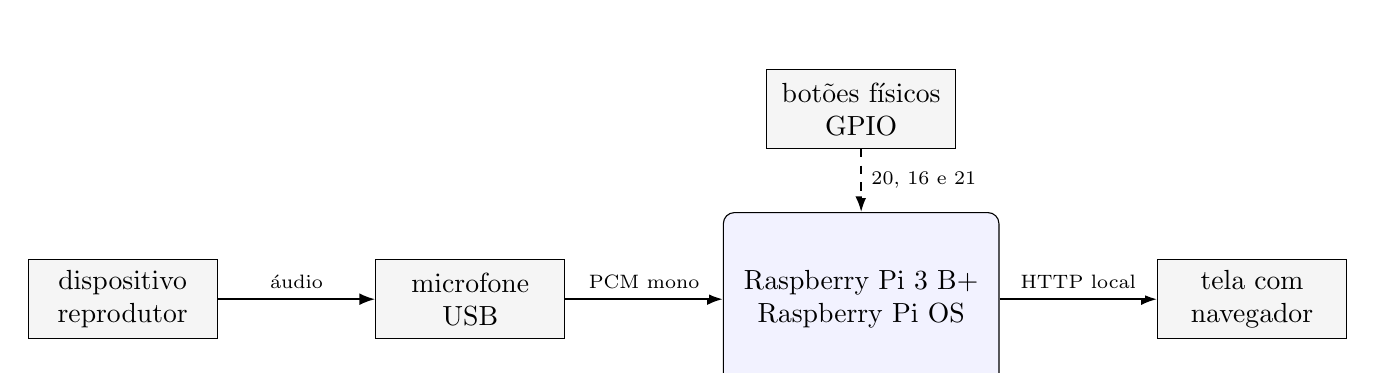
\begin{tikzpicture}[
    node distance=8mm and 20mm,
    bloco/.style={draw, rounded corners, align=center, minimum height=11mm,
        minimum width=27mm, fill=blue!5},
    perif/.style={draw, align=center, minimum height=10mm,
        minimum width=24mm, fill=gray!8},
    fluxo/.style={-{Latex[length=2mm]}, thick},
    controle/.style={-{Latex[length=2mm]}, thick, dashed}
]
    \node[perif] (fonte) {dispositivo\\reprodutor};
    \node[perif, right=of fonte] (microfone) {microfone\\USB};
    \node[bloco, right=of microfone, minimum width=35mm,
        minimum height=22mm] (raspberry) {Raspberry Pi 3 B+\\Raspberry Pi OS};
    \node[perif, above=of raspberry] (botoes) {botões físicos\\GPIO};
    \node[perif, right=of raspberry] (navegador) {tela com\\navegador};

    \draw[fluxo] (fonte) -- node[above, font=\scriptsize, fill=white] {áudio} (microfone);
    \draw[fluxo] (microfone) -- node[above, font=\scriptsize, fill=white] {PCM mono} (raspberry);
    \draw[controle] (botoes) -- node[right, font=\scriptsize, fill=white] {20, 16 e 21} (raspberry);
    \draw[fluxo] (raspberry) -- node[above, font=\scriptsize, fill=white] {HTTP local} (navegador);
\end{tikzpicture}
}
    \caption{Arquitetura física do protótipo. Fonte: elaboração própria.}
    \label{fig:arquitetura-fisica}
\end{figure}

\subsection{Arquitetura estática de software}

A aplicação é dividida entre apresentação, coordenação, processamento e dados,
conforme a Figura~\ref{fig:arquitetura-software}. O navegador envia ações e lê o
estado em JSON; o Flask expõe as rotas; \codigo{RecognitionService} coordena
\emph{threads}, estados e subprocessos; \codigo{GPIOController} converte bordas
de descida em ações; e módulos especializados processam o áudio. O SQLite é
adequado ao catálogo local por ser incorporado ao processo, transacional e não
exigir servidor separado \cite{sqlite2026}.

\begin{figure}[H]
    \centering
    \resizebox{\textwidth}{!}{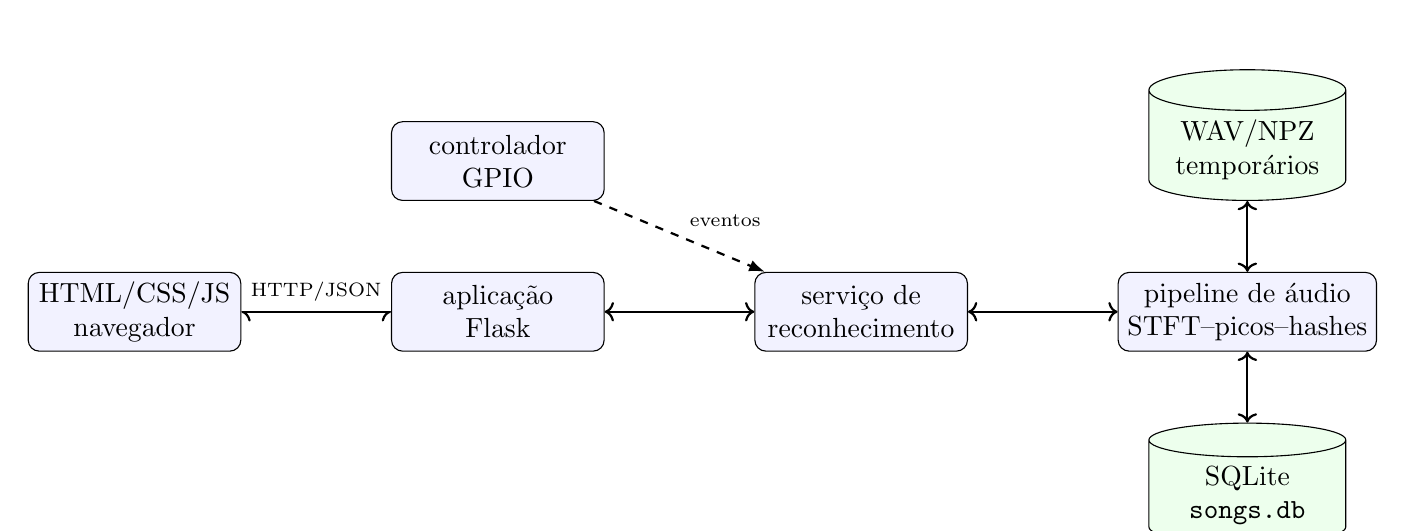
\begin{tikzpicture}[
    node distance=9mm and 19mm,
    componente/.style={draw, rounded corners, align=center, minimum height=10mm,
        minimum width=27mm, fill=blue!5},
    dado/.style={draw, cylinder, shape border rotate=90, aspect=.25,
        align=center, minimum height=12mm, minimum width=25mm, fill=green!7},
    fluxo/.style={-{Latex[length=2mm]}, thick},
    evento/.style={-{Latex[length=2mm]}, thick, dashed}
]
    \node[componente] (browser) {HTML/CSS/JS\\navegador};
    \node[componente, right=of browser] (flask) {aplicação\\Flask};
    \node[componente, above=of flask] (gpio) {controlador\\GPIO};
    \node[componente, right=of flask] (service) {serviço de\\reconhecimento};
    \node[componente, right=of service] (pipeline) {pipeline de áudio\\STFT--picos--hashes};
    \node[dado, below=of pipeline] (db) {SQLite\\\texttt{songs.db}};
    \node[dado, above=of pipeline] (arquivos) {WAV/NPZ\\temporários};

    \draw[fluxo, <->] (browser) -- node[above, font=\scriptsize, fill=white] {HTTP/JSON} (flask);
    \draw[fluxo, <->] (flask) -- (service);
    \draw[evento] (gpio) -- node[above right, font=\scriptsize, fill=white] {eventos} (service);
    \draw[fluxo, <->] (service) -- (pipeline);
    \draw[fluxo, <->] (pipeline) -- (db);
    \draw[fluxo, <->] (pipeline) -- (arquivos);
\end{tikzpicture}
}
    \caption{Arquitetura estática de software. Fonte: elaboração própria.}
    \label{fig:arquitetura-software}
\end{figure}

O navegador consulta \codigo{/api/state} a cada 500 ms. Para uma única interface
na rede local, esse \emph{polling} de duas requisições por segundo simplifica a
sincronização e tem custo pequeno. Em uma evolução com mais clientes, eventos
enviados pelo servidor (SSE) ou WebSocket evitariam consultas repetidas e
reduziriam mensagens no terminal.

\subsection{Arquitetura comportamental}

O fluxo de estados é apresentado na Figura~\ref{fig:fluxo}. O botão azul inicia
uma gravação assíncrona de oito segundos. Ao final, o estado muda para
\codigo{ready}; o verde inicia STFT, picos, fingerprints e matching. O vermelho
pode ser acionado durante gravação ou processamento: o identificador da execução
é invalidado, o grupo do subprocesso recebe \codigo{SIGTERM} e, se não encerrar
em 0,5 s, recebe \codigo{SIGKILL}. Isso impede que uma thread antiga publique um
resultado depois do cancelamento.

\begin{figure}[H]
    \centering
    \resizebox{0.95\textwidth}{!}{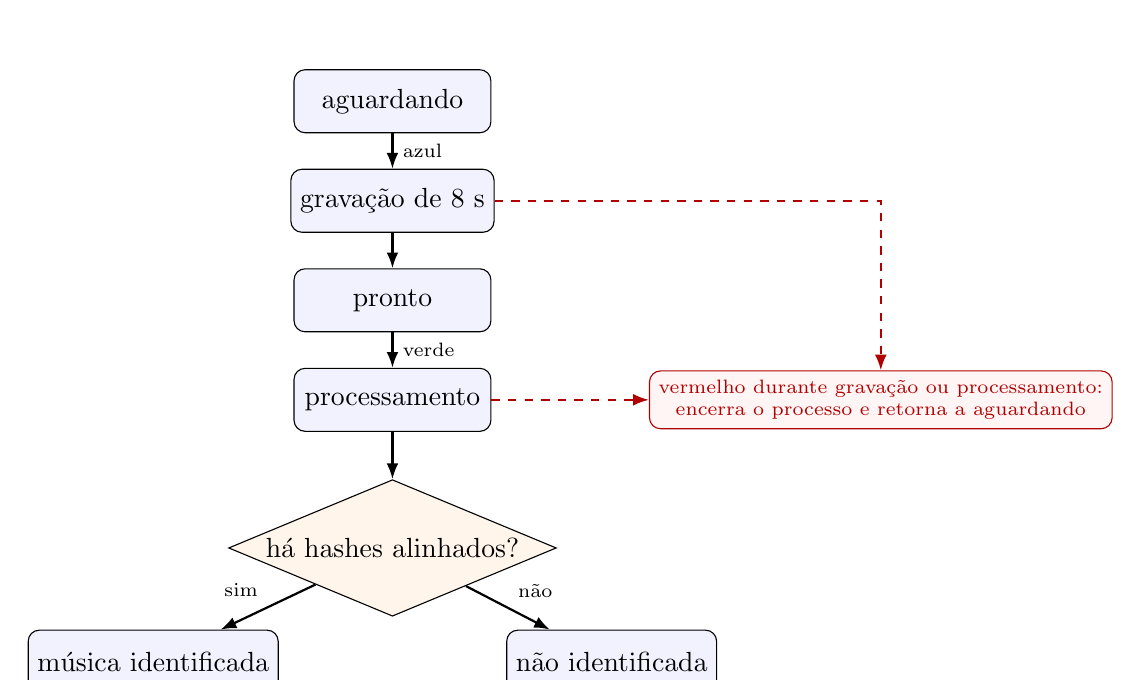
\begin{tikzpicture}[
    node distance=4.5mm and 9mm,
    estado/.style={draw, rounded corners, align=center, minimum height=8mm,
        minimum width=25mm, fill=blue!5},
    decisao/.style={draw, diamond, aspect=2.4, align=center, fill=orange!8,
        inner sep=1.5pt},
    aviso/.style={draw=red!70!black, rounded corners, align=center,
        minimum width=42mm, fill=red!4, text=red!70!black,
        font=\scriptsize},
    fluxo/.style={-{Latex[length=2mm]}, thick},
    cancelar/.style={-{Latex[length=2mm]}, thick, red!70!black, dashed}
]
    \node[estado] (idle) {aguardando};
    \node[estado, below=of idle] (recording) {gravação de 8 s};
    \node[estado, below=of recording] (ready) {pronto};
    \node[estado, below=of ready] (processing) {processamento};
    \node[decisao, below=6mm of processing] (match) {há hashes alinhados?};
    \node[estado, below left=6mm and 4mm of match] (matched) {música identificada};
    \node[estado, below right=6mm and 4mm of match] (nomatch) {não identificada};
    \node[aviso, right=20mm of processing] (cancel) {vermelho durante gravação ou processamento:\\
        encerra o processo e retorna a aguardando};

    \draw[fluxo] (idle) -- node[right, font=\scriptsize] {azul} (recording);
    \draw[fluxo] (recording) -- (ready);
    \draw[fluxo] (ready) -- node[right, font=\scriptsize] {verde} (processing);
    \draw[fluxo] (processing) -- (match);
    \draw[fluxo] (match) -- node[above left, font=\scriptsize] {sim} (matched);
    \draw[fluxo] (match) -- node[above right, font=\scriptsize] {não} (nomatch);
    \draw[cancelar] (recording.east) -| (cancel.north);
    \draw[cancelar] (processing.east) -- (cancel.west);
\end{tikzpicture}
}
    \caption{Fluxo comportamental do reconhecimento. Fonte: elaboração própria.}
    \label{fig:fluxo}
\end{figure}

\section{Implementação}

\subsection{Ferramentas, linguagens e hardware}

Foram usados Raspberry Pi 3 B+, microfone USB, cartão microSD e botões conectados
ao GPIO. O software foi escrito em Python 3 sobre Raspberry Pi OS. NumPy fornece
os vetores numéricos; SciPy, a reamostragem, STFT e filtros de máximos; Matplotlib,
os gráficos; ALSA/\codigo{arecord}, a captura; FFmpeg, a conversão de referências;
SQLite, a persistência; Flask, a interface HTTP; e HTML, CSS e JavaScript, a
apresentação \cite{numpy2026,scipy2026,flask2026}. Git e GitHub foram usados para
versionamento e releases.

\subsection{Organização dos arquivos}

As responsabilidades principais aparecem na Tabela~\ref{tab:modulos}. Artefatos
de referência e consulta são mantidos em diretórios separados, o que facilita
testes e diagnóstico.

\begin{table}[H]
    \centering
    \caption{Principais diretórios e módulos.}
    \label{tab:modulos}
    \small
    \begin{tabularx}{\textwidth}{p{4.7cm} Y}
        \toprule
        \textbf{Caminho} & \textbf{Responsabilidade}\\
        \midrule
        \caminho{src/audio_utils.py} & Conversão, mono, remoção de DC,
        reamostragem e normalização.\\
        \caminho{src/generate_spectrogram.py} & STFT, espectrograma e arquivos NPZ.\\
        \caminho{src/detect_peaks.py} & Máximos locais e mapa de constelação.\\
        \caminho{src/generate_fingerprints.py} & Pareamento de picos e hashes.\\
        \caminho{src/match_song.py} & Busca SQLite e votação de offsets.\\
        \caminho{src/add_song.py} & Conversão e cadastro ou substituição de músicas.\\
        \caminho{src/interface/} & Flask, serviço concorrente, GPIO e páginas web.\\
        \caminho{database/} & Banco SQLite e artefatos numéricos processados.\\
        \caminho{reference_songs/} & Arquivos de áudio de referência.\\
        \caminho{plots/} & Espectrogramas e landmarks para inspeção.\\
        \caminho{tests/} & Testes unitários, integração e benchmark.\\
        \bottomrule
    \end{tabularx}
\end{table}

\subsection{Cadastro e modelo de dados}

O script \codigo{add\_song.py} recebe um arquivo aceito pelo FFmpeg, título,
artista e capa opcional. Ele converte o áudio para WAV PCM mono a 16 kHz, executa
o pipeline e insere tudo em uma transação. A opção \codigo{--replace} preserva o
identificador da música, apaga fingerprints antigos e grava o novo conjunto. O
banco possui a relação \codigo{songs(id, title, artist, album, cover\_file)} e a
relação \codigo{fingerprints(hash, song\_id, offset)}, com índices por hash e por
música. A interface usa um quadro simples com nota musical quando não há capa,
evitando depender de imagens externas.

Ao final, havia 11 músicas e 300.057 fingerprints (Tabela~\ref{tab:banco}).

\begin{table}[H]
    \centering
    \caption{Conteúdo final do banco de fingerprints.}
    \label{tab:banco}
    \small
    \begin{tabularx}{\textwidth}{C{0.7cm} Y Y r}
        \toprule
        \textbf{ID} & \textbf{Título} & \textbf{Artista} & \textbf{Fingerprints}\\
        \midrule
        1 & Espresso & Sabrina Carpenter & 24.853\\
        2 & One True Love & Patrick Patrikios & 19.531\\
        3 & I'm a Believer & Smash Mouth & 26.314\\
        4 & I Can See You & Taylor Swift & 40.021\\
        5 & I Think We're Alone Now & Tiffany & 33.069\\
        6 & Faint & Linkin Park & 23.646\\
        7 & Never Gonna Give You Up & Rick Astley & 31.189\\
        8 & Femininomenon & Chappell Roan & 28.864\\
        9 & Miku & Hatsune Miku & 31.091\\
        10 & Alas & Karol Sevilla & 12.441\\
        11 & Claroscuro & Valentina Zenere & 29.038\\
        \midrule
        \multicolumn{3}{r}{\textbf{Total}} & \textbf{300.057}\\
        \bottomrule
    \end{tabularx}
\end{table}

\subsection{Interface}

A página inicial apresenta o projeto e a página de reconhecimento concentra o
estado, os controles e o cartão de resultado. Quando há identificação, são
exibidos título, artista, capa (ou substituto gráfico) e votos alinhados. A antiga
porcentagem de confiança foi retirada da interface por não representar uma
probabilidade calibrada de acerto; sua exibição poderia induzir uma interpretação
estatística incorreta. O cartão foi dimensionado para a tela do protótipo sem
reduzir o espaçamento de identidade visual no cabeçalho.

\section{Metodologia de desenvolvimento}

Adotou-se desenvolvimento incremental durante quatro ciclos semanais. Cada ciclo
produziu código executável, documentação no README e histórico no Git. O
repositório público está disponível em
\url{https://github.com/ana-vitoria-murad/PCS3732_project}.

\begin{table}[H]
    \centering
    \caption{Síntese dos incrementos.}
    \label{tab:incrementos}
    \small
    \begin{tabularx}{\textwidth}{p{2.2cm} p{2.2cm} Y}
        \toprule
        \textbf{Data/release} & \textbf{Foco} & \textbf{Entrega principal}\\
        \midrule
        29/07, v0.1.0 & Base do sinal & Captura, inspeção de áudio, utilitários,
        espectrograma e banco inicial.\\
        05/08, v0.2.0 & Pipeline completo & Cadastro automático, novas músicas,
        matching, resultados iniciais e documentação.\\
        12/08, v0.3.0 & Integração & Interface web, protótipo visual, GPIO e
        evidências em vídeo.\\
        19/08, ciclo final & Robustez & Cancelamento imediato, ajustes visuais,
        catálogo com 11 músicas e testes automatizados.\\
        \bottomrule
    \end{tabularx}
\end{table}

As decisões foram verificadas primeiro em módulos isolados e depois integradas.
Gráficos de espectrogramas e landmarks ajudaram a inspecionar parâmetros; testes
com arquivos WAV evitaram depender do microfone durante regressões; e a validação
final no hardware verificou a interação física. Essa separação reduziu o custo de
diagnóstico quando uma falha podia estar na aquisição, no processamento ou no
controle da interface.

\section{Testes e resultados}
\label{sec:testes}

\subsection{Estratégia e rastreabilidade}

Foram combinados testes automatizados reprodutíveis e ensaios manuais no hardware.
Os testes automáticos usam referências WAV, não acessam o microfone, não alteram o
banco de produção e aplicam sementes fixas ao ruído. A Tabela~\ref{tab:rastreio}
relaciona casos, requisitos e evidências.

\begin{longtable}{C{1.0cm} p{5.0cm} p{3.0cm} p{4.7cm}}
    \caption{Rastreabilidade entre testes e requisitos.}\label{tab:rastreio}\\
    \toprule
    \textbf{Teste} & \textbf{Procedimento e resultado esperado} &
    \textbf{Requisitos} & \textbf{Evidência}\\
    \midrule
    \endfirsthead
    \toprule
    \textbf{Teste} & \textbf{Procedimento e resultado esperado} &
    \textbf{Requisitos} & \textbf{Evidência}\\
    \midrule
    \endhead
    \bottomrule
    \endfoot
    T01 & Gravar 8 s por USB e obter WAV válido. & RF01, RNF03 &
    Demonstração integrada no hardware.\\
    T02 & Cadastrar/substituir música e preservar ID e metadados. &
    RF02, RF03, RNF04 & \caminho{test_add_song.py}.\\
    T03 & Reconhecer trecho limpo central de cada uma das 11 músicas. &
    RF03--RF06 & \caminho{test_audio_pipeline.py}.\\
    T04 & Avaliar três posições sob condições limpa, ruído e eco. &
    RF04--RF06 & \caminho{benchmark_recognition.py}.\\
    T05 & Submeter silêncio e esperar rejeição antes do matching. & RF07 &
    Teste automatizado aprovado.\\
    T06 & Submeter ruído, tom e acorde sintéticos e esperar ausência de match. &
    RF07 & Falha conhecida documentada.\\
    T07 & Acionar azul, verde e vermelho no GPIO. & RF01, RF06, RF08, RNF03 &
    Ensaio manual na apresentação.\\
    T08 & Cancelar subprocesso ativo e impedir resultado tardio. & RF08 &
    \caminho{test_cancellation.py}.\\
    T09 & Executar sem APIs ou banco remoto. & RNF01 &
    Inspeção da arquitetura e demonstração local.\\
    T10 & Medir captura--resultado na Raspberry Pi. & RNF02 &
    Medição sistemática ainda pendente.\\
    T11 & Inspecionar módulos, documentação e histórico. & RNF05 &
    Código-fonte, README, testes e releases.\\
\end{longtable}

\subsection{Suíte automatizada}

Em 21 de agosto de 2026, a suíte executou seis testes em 1,595 s no ambiente de
desenvolvimento: cinco passaram e um foi registrado como falha esperada. Os casos
aprovados cobrem substituição de música, reconhecimento das 11 referências, ruído
determinístico, rejeição de silêncio e cancelamento de subprocesso. A falha
esperada documenta RF07 até a introdução de um critério mínimo de aceitação.

O benchmark gerou 99 casos de músicas registradas: 11 músicas, três posições
relativas (20\%, 50\% e 80\%) e três condições. Cada trecho tinha oito segundos.
A Tabela~\ref{tab:benchmark} apresenta o resultado obtido no ambiente de
desenvolvimento; o tempo inclui a extração e a consulta em memória, mas não a
captura pelo microfone e não deve ser confundido com a medição de RNF02 no
hardware-alvo.

\begin{table}[H]
    \centering
    \caption{Resultado do benchmark automatizado.}
    \label{tab:benchmark}
    \begin{tabular}{lrrr}
        \toprule
        \textbf{Condição} & \textbf{Corretos} & \textbf{Tempo médio} &
        \textbf{Votos médios}\\
        \midrule
        Limpo & 33/33 & 0,124 s & 942,1\\
        Ruído (SNR de 20 dB) & 33/33 & 0,118 s & 716,5\\
        Eco sintético & 33/33 & 0,118 s & 481,2\\
        \midrule
        \textbf{Total} & \textbf{99/99} & --- & ---\\
        \bottomrule
    \end{tabular}
\end{table}

O teste mede acurácia dentro do catálogo com trechos derivados digitalmente das
próprias referências. Portanto, 100\% nesses 99 casos não implica 100\% em qualquer
ambiente acústico. A queda de votos de áudio limpo para eco mostra que a
perturbação reduz a evidência mesmo quando o vencedor permanece correto.

\subsection{Áudio desconhecido e versões diferentes}

Nos três casos sintéticos desconhecidos, nenhum foi rejeitado: ruído branco foi
associado a \emph{Alas} com dois votos, o tom de 440 Hz a \emph{One True Love}
com um voto e o acorde sintético à mesma música com dois votos. O matcher atual
seleciona o maior agrupamento sempre que existe pelo menos uma colisão; sem limiar
absoluto, razão entre primeiro e segundo colocados ou calibração por densidade,
colisões esparsas podem produzir falso positivo.

Um ensaio complementar foi realizado na apresentação final com três gravações de
\emph{I'm a Believer}: a versão cadastrada no banco, uma versão cover e uma
interpretação de outro artista. Apenas a versão cadastrada foi reconhecida. O
resultado é coerente com o escopo: arranjo, timbre e gravação distintos alteram os
picos e hashes, ainda que a composição seja a mesma. Esse ensaio é uma evidência
negativa útil, mas não elimina a falha observada com sinais sintéticos; são
conjuntos de teste diferentes.

\subsection{Evidências manuais}

Nos testes iniciais, cinco gravações reproduzidas e capturadas pelo microfone
foram identificadas corretamente (Tabela~\ref{tab:manual}). A porcentagem de
confiança do protótipo inicial não é reproduzida porque não era calibrada e foi
removida da interface final.

\begin{table}[H]
    \centering
    \caption{Resultados manuais iniciais.}
    \label{tab:manual}
    \begin{tabularx}{\textwidth}{Y C{2.2cm} r r}
        \toprule
        \textbf{Música} & \textbf{Resultado} & \textbf{Votos} &
        \textbf{Offset}\\
        \midrule
        I'm a Believer & Correto & 25 & 22,9 s\\
        I Think We're Alone Now & Correto & 3 & 60,5 s\\
        I Can See You & Correto & 31 & 167,9 s\\
        Espresso & Correto & 19 & 20,1 s\\
        One True Love & Correto & 3 & 30,7 s\\
        \bottomrule
    \end{tabularx}
\end{table}

As evidências audiovisuais disponíveis são:

\begin{itemize}
    \item \href{https://drive.google.com/file/d/1WVeXX_BBBwl9FQLqkDflyXSvk02ixFJV/view?usp=drive_link}{reconhecimento de \emph{I Think We're Alone Now}};
    \item \href{https://drive.google.com/file/d/1dMfCgbtVWppEejYeSiKkwlpFuSDm9pZl/view?usp=drive_link}{reconhecimento de \emph{I Can See You}}; e
    \item demonstração comparativa de \emph{I'm a Believer}: \VideoFinalURL.
\end{itemize}

\subsection{Situação final dos requisitos}

\begin{table}[H]
    \centering
    \caption{Avaliação final dos requisitos.}
    \label{tab:status}
    \small
    \begin{tabularx}{\textwidth}{p{1.4cm} p{2.5cm} Y}
        \toprule
        \textbf{ID} & \textbf{Situação} & \textbf{Justificativa}\\
        \midrule
        RF01--RF06 & Atendidos & Pipeline completo, cinco ensaios físicos e
        99/99 casos registrados no benchmark.\\
        RF07 & Parcial & Silêncio e duas versões musicais foram rejeitados,
        porém 0/3 sinais sintéticos desconhecidos foram rejeitados.\\
        RF08 & Atendido & Azul, verde e vermelho integrados; cancelamento possui
        teste automatizado. Amarelo é apenas visual e inativo.\\
        RNF01 & Atendido & Processamento, dados e interface são locais.\\
        RNF02 & Inconclusivo & O processamento automatizado foi rápido no ambiente
        de desenvolvimento, mas falta cronômetro da cadeia completa na Pi.\\
        RNF03 & Atendido & Protótipo integrado demonstrado em Raspberry Pi 3.\\
        RNF04 & Atendido & Quatro novas músicas foram incluídas por
        \codigo{add\_song.py}, sem mudar o pipeline.\\
        RNF05 & Atendido qualitativamente & Módulos coesos, docstrings, testes e
        histórico incremental; não foram calculadas métricas estáticas formais.\\
        \bottomrule
    \end{tabularx}
\end{table}

\section{Conclusões}

O Melody atingiu o objetivo central de capturar um trecho, extrair fingerprints,
consultar um catálogo local e apresentar a identificação em uma Raspberry Pi 3.
A integração entre processamento de sinais, SQLite, Flask e GPIO produziu um
protótipo utilizável e inteiramente offline. O cadastro automatizado levou o banco
a 11 músicas sem mudanças no código, e a suíte com 99 casos confirmou regressão
positiva nas três condições avaliadas.

Os resultados também mostram por que acerto dentro do catálogo e rejeição de
desconhecidos são problemas diferentes. O alinhamento temporal identifica bem as
referências, mas o sistema ainda não possui evidência estatística suficiente para
transformar poucos votos em uma decisão de “não reconhecido”. Por esse motivo,
RF07 permanece apenas parcialmente atendido e RNF02 necessita uma medição fim a
fim no hardware. Essa apresentação transparente das limitações evita atribuir à
solução uma robustez que os testes não demonstraram.

As principais dificuldades foram calibrar picos para gravações acústicas,
organizar subprocessos sem bloquear a interface, garantir cancelamento imediato
e conciliar GPIO real com testes executados fora da Raspberry Pi. Como aprendizado,
destacam-se a importância de separar módulos puros de dependências físicas, usar
casos determinísticos para regressão e testar também entradas que não deveriam
ser reconhecidas.

Como trabalhos futuros, recomenda-se: coletar um conjunto maior de negativos
reais; calibrar um limiar por número de votos, margem entre candidatos e quantidade
de fingerprints; medir latência completa e consumo de recursos na Raspberry Pi;
substituir o polling por SSE se houver múltiplos clientes; ampliar o catálogo; e
avaliar parâmetros de picos em ambientes e posições de microfone variados.

\clearpage
\begin{thebibliography}{99}

\bibitem{cooley1965}
COOLEY, James W.; TUKEY, John W. An algorithm for the machine calculation of
complex Fourier series. \textbf{Mathematics of Computation}, Providence, v. 19,
n. 90, p. 297--301, 1965. DOI: 10.1090/S0025-5718-1965-0178586-1.

\bibitem{flask2026}
PALLETS PROJECTS. \textbf{Flask documentation}. Disponível em:
\url{https://flask.palletsprojects.com/en/stable/}. Acesso em: 21 ago. 2026.

\bibitem{numpy2026}
NUMPY DEVELOPERS. \textbf{NumPy documentation}. Disponível em:
\url{https://numpy.org/doc/stable/}. Acesso em: 21 ago. 2026.

\bibitem{raspberry2026}
RASPBERRY PI LTD. \textbf{Raspberry Pi 3 Model B+: product brief}. Cambridge,
s.d. Disponível em:
\url{https://pip-assets.raspberrypi.com/categories/532-raspberry-pi-3-model-b/documents/RP-008338-DS/raspberry-pi-3-b-plus-product-brief.pdf}.
Acesso em: 21 ago. 2026.

\bibitem{scipy2026}
SCIPY COMMUNITY. \textbf{SciPy API reference}. Disponível em:
\url{https://docs.scipy.org/doc/scipy/reference/}. Acesso em: 21 ago. 2026.

\bibitem{sqlite2026}
SQLITE CONSORTIUM. \textbf{About SQLite}. Disponível em:
\url{https://www.sqlite.org/about.html}. Acesso em: 21 ago. 2026.

\bibitem{usp2026}
UNIVERSIDADE DE SÃO PAULO. \textbf{PCS3732 --- Laboratório de Processadores}.
JúpiterWeb. Disponível em:
\url{https://uspdigital.usp.br/jupiterweb/obterDisciplina?sgldis=PCS3732&verdis=2}.
Acesso em: 21 ago. 2026.

\bibitem{wang2003}
WANG, Avery Li-Chun. An industrial-strength audio search algorithm. In:
\textbf{INTERNATIONAL CONFERENCE ON MUSIC INFORMATION RETRIEVAL}, 4., 2003,
Baltimore. \textbf{Proceedings [...]} Baltimore: ISMIR, 2003. p. 7--13.
Disponível em: \url{https://zenodo.org/records/1416340}. Acesso em: 21 ago. 2026.

\end{thebibliography}

\appendix
\clearpage
\section{Comandos de reprodução}

Os comandos abaixo devem ser executados a partir da pasta
\codigo{song-recognizer}, após ativar o ambiente virtual e instalar as
dependências do projeto.

\begin{verbatim}
# Testes rápidos
PYTHONPATH=src:. python -m unittest discover -s tests -v

# Benchmark completo
MPLCONFIGDIR=/tmp/melody-mpl PYTHONPATH=src:. \
python tests/benchmark_recognition.py

# Interface local com GPIO
sudo pigpiod
MELODY_ENABLE_GPIO=1 MELODY_AUDIO_DEVICE=plughw:2,0 \
PYTHONPATH=. python src/interface/app.py

# Cadastro de música
PYTHONPATH=src:. python src/add_song.py caminho/musica.mp3 \
  --title "Título" --artist "Artista"
\end{verbatim}

\end{document}
